\documentclass[11pt,a4paper]{article}

% ─── Packages ────────────────────────────────────────────────────
\usepackage[utf8]{inputenc}
\usepackage[T1]{fontenc}
\usepackage{lmodern}
\usepackage[margin=1in]{geometry}
\usepackage{amsmath,amssymb,amsfonts}
\usepackage{graphicx}
\usepackage{booktabs}
\usepackage{hyperref}
\usepackage{xcolor}
% natbib removed — using manual thebibliography instead
\usepackage{caption}
\usepackage{subcaption}
\usepackage{float}
\usepackage{enumitem}
\usepackage{microtype}
\usepackage{authblk}

\hypersetup{
    colorlinks=true,
    linkcolor=blue!60!black,
    citecolor=blue!60!black,
    urlcolor=blue!60!black
}

% ─── Title ───────────────────────────────────────────────────────
\title{%
  \textbf{Verdant-Minds: A Hybrid Cognitive Architecture\\
  with Graph Memory, Wave-State Dynamics,\\
  and Measurable Emergent Concept Scaffolding}%
}

\author[1]{William Adams}
\affil[1]{Independent Researcher}
\date{March 2026}

% ─── Document ────────────────────────────────────────────────────
\begin{document}
\maketitle

% ─── Abstract ────────────────────────────────────────────────────
\begin{abstract}
Verdant-Minds is a research-grade cognitive architecture that processes text 
through a structured nine-stage pipeline (sensory $\to$ pattern $\to$ memory 
$\to$ communication $\to$ reasoning $\to$ ethics $\to$ action $\to$ language 
$\to$ learning). The system maintains a symbolic MemoryWeb (graph memory) 
coupled bidirectionally to an Extended Cognitive Wave Function (ECWF), a 
compact, configurable wave-state model whose entropy, magnitude, and phase 
influence memory reinforcement, decay, and concept formation. A governance 
layer (``Three Kings'') provides oversight across data quality, ethics, and 
action selection.

We report evidence from cultivation runs that emergent concepts---concepts 
created autonomously by the system's wave dynamics rather than seeded by 
designers---not only appear, but preferentially link to earlier emergent 
concepts in the memory backbone. In a representative run (119 concepts, 37 
emergent nodes), emergent$\to$emergent edges in a sparsified backbone exhibit 
a strong timing bias toward linking newer emergents to older emergents 
(observed earlier-share 0.807; shuffle baseline $\sim$0.499$\pm$0.083; 
$z \approx 3.71$), suggesting temporal scaffolding during concept formation. 
These results are not claims of consciousness; they are measurable structural 
properties of an evolving concept graph coupled to a state-dynamics core.
\end{abstract}

\vspace{1em}
\noindent\textbf{Keywords:} cognitive architecture, emergent concepts, graph memory, 
wave-state dynamics, ethomorphism, temporal scaffolding

% ─── 1. Motivation ───────────────────────────────────────────────
\section{Motivation}

Modern AI systems are dominated by large neural models that are powerful but 
opaque. Verdant-Minds explores an alternate route: a modular cognitive pipeline 
with explicit memory, governance, and measurable internal state dynamics. The 
goal is not to replace large language models but to create an architecture where:

\begin{itemize}[nosep]
    \item memory is explicit and inspectable,
    \item ethics and action gating are first-class processing stages,
    \item internal state evolution can be instrumented and measured,
    \item and emergent structure can be observed and quantified over time.
\end{itemize}

The project is developed under the banner of \textit{Ethomorphic AI}---the 
principle that ethical reasoning is geometrically embedded in cognitive state 
space rather than applied as an external constraint. Verdant-Minds is the 
first implementation of this principle.

% ─── 2. System Overview ─────────────────────────────────────────
\section{System Overview}

Verdant-Minds is organized as five interacting subsystems:

\begin{enumerate}[nosep]
    \item \textbf{Nine-block cognitive pipeline}: deterministic sequencing of 
          processing stages from sensory input through continual learning.
    \item \textbf{MemoryWeb}: graph-based concept memory with reinforcement, 
          decay, and spreading activation retrieval.
    \item \textbf{ECWF core}: multi-facet complex-valued wave state 
          representing cognitive and ethical dimensions; produces entropy, 
          magnitude, and phase signals.
    \item \textbf{Memory\texorpdfstring{$\leftrightarrow$}{-}ECWF Bridge}: bidirectional coupling 
          where memory influences wave parameters and wave outputs reinforce 
          memory and generate new concepts.
    \item \textbf{Three Kings governance}: oversight and conflict resolution 
          at key points in the pipeline.
\end{enumerate}

This architecture is designed to be inspected, instrumented, and adapted---closer 
in lineage to cognitive architectures such as SOAR~\cite{laird2012soar}, 
ACT-R~\cite{anderson2004actr}, and OpenCog~\cite{goertzel2014opencog} than 
to chat-style applications.

% ─── 3. Architecture Details ────────────────────────────────────
\section{Architecture Details}

\subsection{Nine-Block Pipeline}

Each input is wrapped into a shared state container (CognitiveChunk) that 
accumulates sections and a processing log. Blocks read prior sections and 
write their own, yielding a traceable per-input ``cognitive episode.''

The processing order is: Sensory Input $\to$ Pattern Recognition $\to$ Memory 
Storage $\to$ Internal Communication $\to$ Reasoning \& Planning $\to$ Ethics 
\& Values $\to$ Action Selection $\to$ Language Processing $\to$ Continual 
Learning. The final block may trigger emergent concept detection.

\subsection{MemoryWeb (Graph Memory)}

MemoryWeb is a concept graph implemented over NetworkX in which nodes store 
stability scores, access counts, timestamps, metadata, and weighted connection 
lists. Edges may be gated by an ethical-distance-dependent probability 
(``pconnect''):

\begin{equation}
    p_{\text{accept}} = (1 - p_{\text{eth}} \cdot \delta_e) \cdot 
    \exp(-\beta_E \cdot \Delta_E), \quad 
    p_{\text{accept}} \in [0, 1]
    \label{eq:pconnect}
\end{equation}

\noindent where $p_{\text{eth}} = 0.6$ and $\beta_E = 1.0$ are default 
constants, $\delta_e$ is a local ethical distance, and $\Delta_E$ is a 
global ethical distance measure. An edge is accepted if a uniform random 
draw falls below $p_{\text{accept}}$.

\subsection{ECWF (Wave-State Core)}

The Extended Cognitive Wave Function represents system state as a sum of 
complex facets:

\begin{equation}
    \Psi(x, e, t) = \sum_{i=1}^{n} M_i(x, e, t) \cdot 
    \exp\!\bigl(j\,(2\pi k_i \cdot x + 2\pi m_i \cdot e - \omega_i t + \phi_i)\bigr)
    \label{eq:ecwf}
\end{equation}

\noindent where $x \in \mathbb{R}^{d_c}$ are cognitive dimensions, 
$e \in \mathbb{R}^{d_e}$ are ethical dimensions, $t$ is time, $M_i$ is the 
amplitude function for facet $i$, $k_i$ and $m_i$ are wave numbers, 
$\omega_i$ is angular frequency, and $\phi_i$ is phase shift. The system 
computes Shannon entropy over $|\Psi|^2$ as an uncertainty signal, and 
numerical sensitivity gradients via finite-difference perturbation.

ECWF also maintains short-horizon history coupling through exponentially 
decayed averaging of past states, enabling dynamic dependence on recent 
cognitive history.

\subsection{\texorpdfstring{Memory$\leftrightarrow$ECWF Bridge}{Memory-ECWF Bridge}}

The bridge performs two-way coupling each processing cycle:

\begin{itemize}[nosep]
    \item \textbf{Memory $\to$ Wave}: active concepts modulate ECWF parameters 
          via influence vectors derived from concept stability and dimension 
          mappings.
    \item \textbf{Wave $\to$ Memory}: wave outputs activate concepts through 
          dimension reverse-lookup, reinforce or decay stability based on 
          thermodynamic phase, and detect conditions for emergent concept 
          creation.
\end{itemize}

Concept-dimension mappings are initialized using sentence-transformer 
embeddings (all-MiniLM-L6-v2) projected via PCA to the ECWF dimension 
space, ensuring that semantically related concepts map to nearby regions 
in the wave function.

\subsection{Governance (``Three Kings'')}

Governance is layered oversight operating at specific pipeline stages:

\begin{itemize}[nosep]
    \item \textbf{Data King}: information quality assessment and anomaly 
          detection (operates at Block 4).
    \item \textbf{Ethics King}: ethical evaluation and response modulation, 
          incorporating coherence tension signals (operates at Block 6).
    \item \textbf{Forefront King}: phase-aware attention allocation, capacity 
          controls, and decision threshold management (operates at Block 7).
\end{itemize}

\noindent The Three Kings Council coordinates conflict resolution for critical 
decisions via weighted influence and consensus mechanisms.

\subsection{Thermodynamic Phase Control}

The system employs a glass-transition temperature parameter ($T_g$) as a 
first-class control signal that modulates processing behavior:

\begin{itemize}[nosep]
    \item \textbf{Rigid} ($T_g < 0.4$): low decay, low reinforcement, high 
          decision thresholds---stabilization behavior.
    \item \textbf{Flexible} ($0.4 \leq T_g \leq 0.6$): balanced 
          exploration/exploitation.
    \item \textbf{Chaotic} ($T_g > 0.6$): high decay, high reinforcement, 
          low decision thresholds---exploratory behavior.
\end{itemize}

\subsection{Coherence Geometry}

Each cycle computes coherence invariants from wave, ethics, and memory 
telemetry. The system constructs a generalized metric 
$\tau_\alpha(a,b) = |a - b|^\alpha$ and checks triangle inequality validity 
across an $\alpha$-grid. The Housed Contradiction Index (HCI) quantifies 
internal cognitive tension. These signals feed back into governance: the 
Forefront King adjusts its decision threshold under coherence strain, and 
the Ethics King modulates its overall score when geometric tension is 
detected.

% ─── 4. Emergent Concept Formation ──────────────────────────────
\section{Emergent Concept Formation}

\subsection{Trigger Conditions}

Emergent concept creation is gated by multiple conditions that must all 
be satisfied simultaneously:

\begin{enumerate}[nosep]
    \item \textbf{Magnitude gate}: wave magnitude must exceed a minimum 
          threshold (default 0.15) at the callsite in the continual learning 
          block.
    \item \textbf{Entropy window}: sensitivity entropy must fall within 
          $[0.3, 3.0]$, rejecting states that are too ordered or too chaotic 
          for meaningful pattern formation.
    \item \textbf{Strength gate}: mean sensitivity magnitude must exceed the 
          detector threshold (default 0.15).
    \item \textbf{Novelty gate}: the combination key (sorted top-3 concept 
          identifiers) must not have been seen before.
\end{enumerate}

When semantic embeddings are available, candidate ranking blends stability 
with inverse semantic similarity (``surprise''). This biases the system 
toward creating concepts that bridge semantically distant parents---non-obvious 
combinations that pure graph proximity would not surface.

\subsection{Creation and Integration}

New emergent concepts are added to the MemoryWeb with structured metadata 
(origin, creation time, entropy, magnitude) and connected to their parent 
concepts. Critically, emergent concepts receive dimension mappings in the 
ECWF space, making them visible to future wave dynamics. This means 
emergent concepts can participate in the activation of subsequent emergent 
concepts, enabling second-order associative structure.

% ─── 5. Experimental Setup ──────────────────────────────────────
\section{Experimental Setup}

\subsection{Cultivation Loop}

An external LLM provider (Groq, Anthropic, or Mistral) acts as a cultivation 
tutor, generating inputs designed to produce cognitive tension in the system. 
The cultivator monitors HCI, phase state, and emergent concept generation. It 
employs a domain rotation wheel (9 domains), phase-aware input selection 
(rigid$\to$depth, flexible$\to$paradox, chaotic$\to$grounding), and forced 
perturbation at configurable intervals to prevent phase plateaus.

Each cycle, the system processes the input through the full nine-block 
pipeline, updates memory and wave state, and logs structured telemetry 
to a JSONL cycle log.

\subsection{Instrumentation}

For each cycle we capture: MemoryWeb size and topology, emergent concept 
count and identities, coherence invariants (HCI, triangle validity, violation 
rate, $\alpha$-critical), thermodynamic phase state, and per-block processing 
metrics. Full system state is persisted as JSON at configurable intervals.

\subsection{Representative Run Parameters}

The results reported below are drawn from a representative cultivation run 
with the following parameters:

\begin{itemize}[nosep]
    \item Seed: 42 (NumPy RNG + ECWF random state)
    \item Cycles: 91
    \item Provider: Groq (llama-3.3-70b-versatile)
    \item Perturbation interval: 15 cycles
    \item ECWF dimensions: 5 cognitive + 5 ethical
    \item Initial knowledge base: 82 seeded concepts across 9 domains
\end{itemize}

% ─── 6. Results ─────────────────────────────────────────────────
\section{Results: Temporal Scaffolding in Emergent Concept Links}

\subsection{Run Summary}

At the conclusion of the representative run:

\begin{itemize}[nosep]
    \item Total concepts: 119 (82 seeded + 37 emergent)
    \item MemoryWeb backbone: 513 edges (top-6 edges per node sparsification)
    \item Self-cluster average access count: 2895.2
    \item Non-self-cluster average access count: 8.4
    \item Access count ratio: 345$\times$
\end{itemize}

\subsection{Key Finding: Preferential Attachment to Earlier Emergent Concepts}

We analyzed emergent$\to$emergent (EE) edges in the sparsified backbone and 
oriented each edge by the creation timestamp embedded in each emergent 
concept's name (newer $\to$ older). We observed:

\begin{table}[H]
\centering
\begin{tabular}{lr}
\toprule
\textbf{Metric} & \textbf{Value} \\
\midrule
Observed earlier-share & 0.807 \\
Shuffle baseline (mean) & $\sim$0.499 \\
Shuffle baseline (std) & $\pm$0.083 \\
$z$-score & $\approx$3.71 \\
\bottomrule
\end{tabular}
\caption{Temporal bias in emergent$\to$emergent link direction. The observed 
earlier-share substantially exceeds the shuffle baseline, indicating that 
newer emergent concepts preferentially link to older emergent concepts 
($p < 0.001$ under the shuffle null).}
\label{tab:scaffolding}
\end{table}

\noindent\textbf{Interpretation}: Emergent concepts in this run linked to 
older emergents substantially more than expected under random timing, 
consistent with a temporal ``scaffolding'' effect in which later concepts 
build upon earlier emergent structure. This is a structural property of the 
evolving concept graph, not a claim about consciousness or understanding.

\subsection{Visual Evidence}

\begin{figure}[H]
    \centering
    \begin{subfigure}[t]{0.55\textwidth}
        \centering
        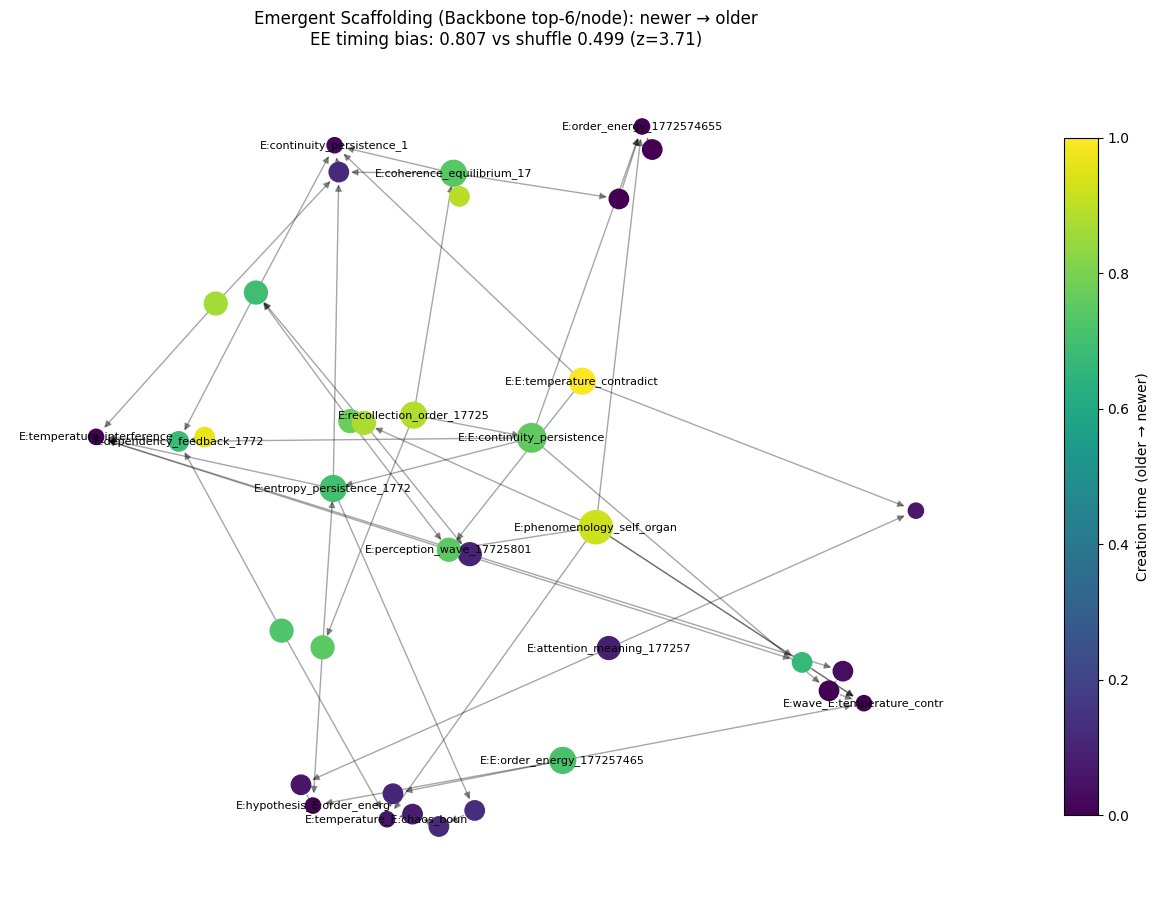
\includegraphics[width=\textwidth]{figures/emergent_scaffolding.png}
        \caption{Emergent scaffold graph (directed newer$\to$older). Node 
        color indicates creation time (dark = early, bright = late). Edge 
        direction shows the temporal orientation of emergent$\to$emergent 
        links in the backbone.}
        \label{fig:scaffold}
    \end{subfigure}
    \hfill
    \begin{subfigure}[t]{0.42\textwidth}
        \centering
        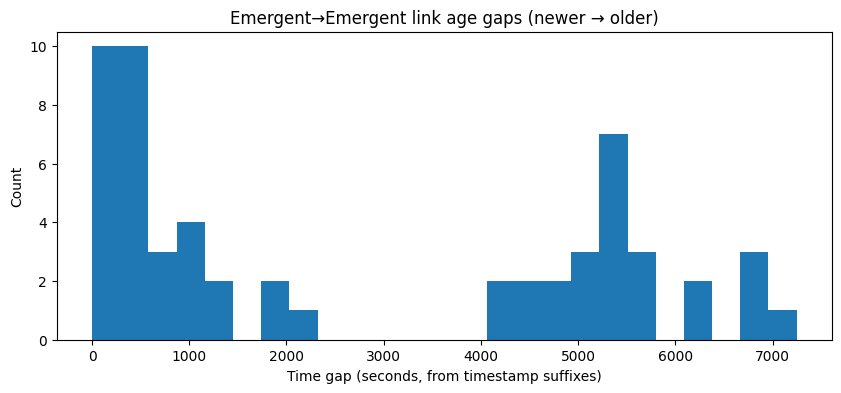
\includegraphics[width=\textwidth]{figures/link_age_gaps.png}
        \caption{Distribution of time gaps (seconds) between linked emergent 
        concepts. The concentration at small gaps ($<$1000s) indicates 
        temporally proximate scaffolding, with a secondary cluster at 
        larger gaps suggesting cross-epoch bridging.}
        \label{fig:agegaps}
    \end{subfigure}
    \caption{Emergent concept scaffolding structure from the representative 
    91-cycle cultivation run.}
    \label{fig:results}
\end{figure}

\noindent\textit{Note}: To reproduce these figures, place the image files in 
a \texttt{figures/} directory as \texttt{emergent\_scaffolding.png} and 
\texttt{link\_age\_gaps\allowbreak.png}.

% ─── 7. Limitations ─────────────────────────────────────────────
\section{Limitations}

We note the following limitations to maintain defensibility:

\begin{enumerate}[nosep]
    \item \textbf{Language output}: The system's language generation block is 
          currently template-based. Output text quality does not reflect the 
          sophistication of internal state dynamics.
    \item \textbf{Naming reliance on timestamps}: Emergent concept naming 
          encodes creation timestamps. Future work should validate temporal 
          ordering against stored \texttt{creation\_time} metadata as the 
          primary source of truth.
    \item \textbf{Single-run evidence}: The scaffolding results are drawn 
          from a representative run. Multi-seed, multi-provider replication 
          with distributional statistics (mean $\pm$ sd) is needed before 
          strong structural claims.
    \item \textbf{No benchmark comparisons}: The architecture has not yet been 
          evaluated against standardized cognitive architecture benchmarks.
    \item \textbf{Dimensional constraints}: The current 5+5 dimensional ECWF 
          space creates concept aliasing at scale. The v2 architecture 
          (in progress) supports configurable dimensionality up to 64+64.
    \item \textbf{Temperature heuristic}: $T_g$ is derived from input 
          complexity features, not from an energy functional. True 
          thermodynamic grounding requires defining $T = (\partial E / 
          \partial S)^{-1}$ over a system energy functional.
\end{enumerate}

% ─── 8. Related Work ────────────────────────────────────────────
\section{Related Work}

Verdant-Minds shares structural elements with several existing frameworks 
while differing in its combination of wave-state dynamics with symbolic 
graph memory.

\textbf{Cognitive architectures}: SOAR~\cite{laird2012soar} and 
ACT-R~\cite{anderson2004actr} provide modular cognitive pipelines with 
explicit memory systems. Verdant differs in its continuous wave-state 
representation and bidirectional bridge between symbolic and subsymbolic 
layers.

\textbf{Global Workspace Theory}: The CognitiveChunk flowing through 
governance-gated blocks resembles the global workspace 
paradigm~\cite{baars1988gwt}, with the Three Kings playing the role 
of attentional gatekeepers.

\textbf{Conceptual Spaces}: The ECWF dimension space where concepts are 
mapped via embeddings is structurally a conceptual 
space~\cite{gardenfors2000conceptual}, with emergent concept formation 
finding novel regions through wave dynamics.

\textbf{Integrated Information Theory}: The coherence geometry---particularly 
HCI and triangle validity checks---attempts something functionally similar 
to IIT's $\Phi$ measure~\cite{tononi2004iit}: quantifying the degree to 
which a system's state is integrated.

The key architectural novelty is the bidirectional bridge between a symbolic 
concept graph and a continuous wave function, with emergent concepts arising 
from wave dynamics and feeding back into the symbolic layer. This combination 
is not present in any of the above frameworks.

% ─── 9. Roadmap ─────────────────────────────────────────────────
\section{Roadmap}

\textbf{Near-term}: Clean packaging (v2 extraction of ethomorphic core as 
separable package), stable chunked persistence, API server and dashboard 
for demonstration, benchmark harnesses.

\textbf{Medium-term}: Multiple-run statistical validation, controlled 
ablations (disable bridge, disable pconnect, vary entropy window), 
dimensional scaling experiments (16+16, 32+32, 64+64).

\textbf{Long-term}: Integration with external reasoning backends (LLM-powered 
language block), application to safety-sensitive domains requiring auditable 
cognition, and exploration of the ethomorphic core as a general-purpose 
module for embedding ethical geometry in other AI systems.

% ─── 10. Conclusion ─────────────────────────────────────────────
\section{Conclusion}

Verdant-Minds demonstrates a modular cognitive architecture with explicit 
memory, governance, and a wave-state core that yields measurable internal 
dynamics. Cultivation runs show not only emergent concept creation but 
evidence of temporal scaffolding among emergent concepts in the MemoryWeb 
backbone. This suggests the system is forming higher-order structure over 
time---an engineering property that can be instrumented, tested, and improved.

The separation of the ethomorphic core (wave engine, bridge, coherence 
geometry, ethical embedding) as an independent package establishes a 
foundation for applying the Ethomorphic AI principle to systems beyond the 
current Verdant architecture.

% ─── Appendix A ─────────────────────────────────────────────────
\appendix
\section{Reproducibility and Implementation Notes}

\subsection{Environment and Entry Points}

The cultivation runner is located at \texttt{scripts/verdant\_llm\_cultivator.py}. 
The core system initializes with a deterministic seed (default: 42) applied to 
NumPy and ECWF random state. Emergence is invoked from the continual learning 
block when wave magnitude exceeds 0.15, then filtered by the detector-level 
entropy window and magnitude threshold.

\subsection{Reproduction Commands}

\begin{verbatim}
pip install -r requirements.txt
export GROQ_API_KEY=...
export GROQ_MODEL=llama-3.3-70b-versatile

# Fresh run
python scripts/verdant_llm_cultivator.py \
  --fresh --max-cycles 120 \
  --max-tokens-per-call 96 \
  --budget-mode light \
  --perturbation-interval 15

# Resume
python scripts/verdant_llm_cultivator.py \
  --resume

# Load explicit state
python scripts/verdant_llm_cultivator.py \
  --load-state \
  outputs/cultivation_state_<stamp>.json
\end{verbatim}

\subsection{Output Artifacts}

A single cultivation run produces timestamped outputs under \texttt{outputs/}:

\begin{itemize}[nosep]
    \item \texttt{cultivation\_cycles\_<stamp>.jsonl} --- per-cycle records
    \item \texttt{cultivation\_state\_<stamp>.json} --- final system state
    \item \texttt{cultivation\_session\_<stamp>.json} --- session summary
    \item \texttt{significant\_events\_<stamp>.json} --- major events
\end{itemize}

\subsection{Emergence Gating Parameters}

\begin{table}[H]
\centering
\begin{tabular}{llr}
\toprule
\textbf{Gate} & \textbf{Condition} & \textbf{Default} \\
\midrule
Callsite magnitude & wave\_magnitude $>$ threshold & 0.15 \\
Entropy window & sensitivity entropy $\in [lo, hi]$ & [0.3, 3.0] \\
Strength gate & mean sensitivity $>$ threshold & 0.15 \\
Novelty gate & combo\_key unseen & --- \\
Surprise criterion & stability $\times$ inverse similarity & optional \\
\bottomrule
\end{tabular}
\caption{Emergence gating conditions and default parameter values.}
\label{tab:gating}
\end{table}

\subsection{Determinism Notes}

Even with a fixed core seed, strict run-to-run equivalence is not guaranteed 
due to: LLM provider nondeterminism, cultivator perturbation timing, and 
external API fallback chains. When reporting structural findings, we recommend 
distributional results across multiple runs (mean $\pm$ sd) rather than 
single-run claims.

\subsection{Minimum Reproducibility Pack}

For full reproducibility, attach: the JSONL cycle log, final state JSON, 
session summary, significant events log, the exact CLI command used, provider 
model string(s), and the git commit hash at run time.

% ─── References ──────────────────────────────────────────────────
\begin{thebibliography}{10}

\bibitem[Anderson et~al.(2004)]{anderson2004actr}
Anderson, J.~R., Bothell, D., Byrne, M.~D., Douglass, S., Lebiere, C., 
\& Qin, Y. (2004).
\newblock An integrated theory of the mind.
\newblock \textit{Psychological Review}, 111(4), 1036--1060.

\bibitem[Baars(1988)]{baars1988gwt}
Baars, B.~J. (1988).
\newblock \textit{A Cognitive Theory of Consciousness}.
\newblock Cambridge University Press.

\bibitem[G{\"a}rdenfors(2000)]{gardenfors2000conceptual}
G{\"a}rdenfors, P. (2000).
\newblock \textit{Conceptual Spaces: The Geometry of Thought}.
\newblock MIT Press.

\bibitem[Goertzel et~al.(2014)]{goertzel2014opencog}
Goertzel, B., Pennachin, C., \& Geiger, N. (2014).
\newblock \textit{Engineering General Intelligence}.
\newblock Atlantis Press.

\bibitem[Laird(2012)]{laird2012soar}
Laird, J.~E. (2012).
\newblock \textit{The Soar Cognitive Architecture}.
\newblock MIT Press.

\bibitem[Tononi(2004)]{tononi2004iit}
Tononi, G. (2004).
\newblock An information integration theory of consciousness.
\newblock \textit{BMC Neuroscience}, 5(1), 42.

\end{thebibliography}

\end{document}
